\newpage
\section{There Are Many Factors to Consider}\label{A:CF}

\fixnote{Revise.  List all factors of several numbers.  Need an example where being systematic by consecutive numbers (rather than by using prime factorization) is inefficient.
List all the factors of 60 with their prime factorization.}  

\begin{prob} How many factors does the integer $60$ have?
\end{prob}

\begin{prob}
Consider the following diagram:
\[
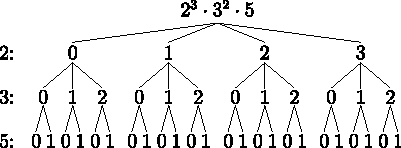
\includegraphics{../graphics/treeDia.pdf}
\]
What is going on in this diagram? What do the numbers represent? How
does it help you count the number of factors of $2^3\cdot 3^2 \cdot
5$?
\end{prob}

\begin{prob}
Make a similar diagram for $60$.
\end{prob}

\begin{prob} 
Can you devise a method for computing the number of factors that a
number has? Explain why your method works.
\end{prob}

\begin{prob} How many factors does $735$ have?
\end{prob}

\begin{prob} 
If $p$ is a prime number, how many factors does $p^n$ have?
\end{prob}

\begin{prob} 
If $p$ and $q$ are both prime numbers, how many factors does $p^nq^m$
have?
\end{prob}

\begin{prob} Which integers between $0$ and $100$ have the most factors?         
\end{prob}
